%
% kugeldreieck.tex
%
% (c) 2021 Prof Dr Andreas Müller, OST Ostschweizer Fachhochschule
%
\documentclass[tikz]{standalone}
\usepackage{times}
\usepackage{amsmath}
\usepackage{txfonts}
\usepackage[utf8]{inputenc}
\usepackage{graphics}
\usetikzlibrary{arrows,intersections,math}
\usepackage{ifthen}
\begin{document}

\newboolean{showgrid}
\setboolean{showgrid}{false}
\def\breite{7}
\def\hoehe{4}

\begin{tikzpicture}[>=latex,thick]

% Povray Bild
\node at (0,0) {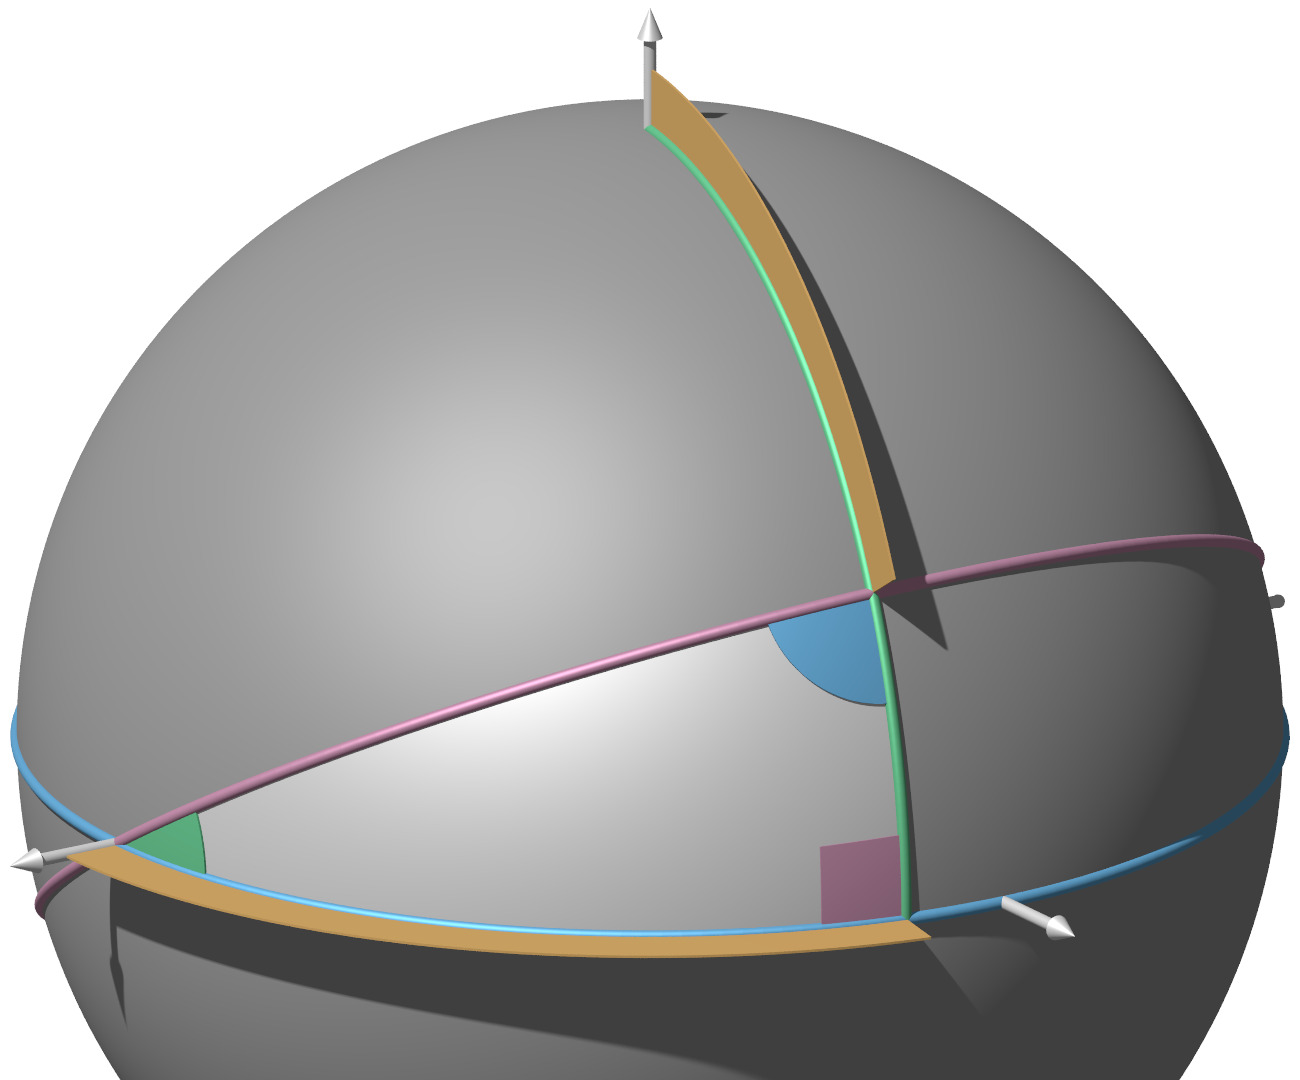
\includegraphics[width=10.0cm]{kugeldreieck.jpg}};

% Gitter
\ifthenelse{\boolean{showgrid}}{
\draw[step=0.1,line width=0.1pt] (-\breite,-\hoehe) grid (\breite, \hoehe);
\draw[step=0.5,line width=0.4pt] (-\breite,-\hoehe) grid (\breite, \hoehe);
\draw                            (-\breite,-\hoehe) grid (\breite, \hoehe);
\fill (0,0) circle[radius=0.05];
}{}

\node at (-4.1,-2) {$A$};
\node at (2,-3.3) {$C$};
\node at (1.4,-0.2) {$B$};

\node at (1.5,-0.9) {$\beta$};
\node at (-3.6,-2.34) {$\alpha$};
\node at (1.1,1.6) [left] {$\vartheta$};
\node at (1.7,-2.7) {$\gamma$};

\node at (-1.1,-0.9) [rotate=19] {$c = t$};
\node at (-1,-2.75) [rotate=-3] {$b = \varphi$};
\node at (2.0,-1.5) [right] {$a=\displaystyle\frac{\pi}2-\vartheta$};

\end{tikzpicture}

\end{document}

